\documentclass[11pt]{article}
\usepackage{amsmath,amssymb,amsfonts}
\usepackage{graphicx}
\usepackage[utf8]{inputenc}
\usepackage{xcolor}
\usepackage{url}
\usepackage[numbers,sort&compress]{natbib}
\usepackage{hyperref}
\usepackage{geometry}
\usepackage{authblk}

\hypersetup{
  pdfauthor={QMCPy Authors},
  pdftitle={QMCPy: An Open-Source Python Framework},
  pdfsubject={Quasi-Monte Carlo},
  pdfkeywords={QMC, Monte Carlo, Python},
  pdfproducer={Pandoc with LaTeX}
}

\geometry{margin=1in}

\hypersetup{
  colorlinks=true,
  linkcolor=blue,
  citecolor=blue,
  urlcolor=blue,
  filecolor=magenta,
  linktoc=all,
  breaklinks=true
}

\usepackage{xspace,titlesec}
\providecommand{\HickernellFJ}{Hickernell\xspace}

% Pandoc compatibility
\providecommand{\tightlist}{%
  \setlength{\itemsep}{0pt}\setlength{\parskip}{0pt}}

% CSL references environment
\newlength{\cslhangindent}
\setlength{\cslhangindent}{1.5em}
\newlength{\csllabelwidth}
\setlength{\csllabelwidth}{3em}
% Suppress the automatic heading by redefining CSLReferences to not add a section
\newenvironment{CSLReferences}[2]
  {\begin{thebibliography}{#1}}
  {\end{thebibliography}}
\newcommand{\CSLBlock}[1]{#1\hfill\break}
\newcommand{\CSLLeftMargin}[1]{\parbox[t]{\csllabelwidth}{#1}}
\newcommand{\CSLRightInline}[1]{\parbox[t]{\linewidth - \csllabelwidth}{#1}\break}
\newcommand{\CSLIndent}[1]{\hspace{\cslhangindent}#1}

% Citation processing commands
\providecommand{\citeproctext}{}
\providecommand{\citeproc}[1]{#1}

% Redefine bibitem to handle empty labels properly
\let\oldbibitem\bibitem
\renewcommand{\bibitem}[2][]{\oldbibitem{#2}}

% Suppress pandoc's automatic reference section heading
\renewcommand{\refname}{}

\title{\textbf{\texttt{QMCPy}}: An Open-Source Python Framework for
(Quasi-)Monte Carlo Algorithms}

\author[1]{Aleksei G. Sorokin}
\author[1]{Fred J. Hickernell}
\author[1, 2]{Sou-Cheng T. Choi}
\author[3]{Jagadeeswaran Rathinavel}
\author[4]{Pieterjan Robbe}
\author[5]{Aadit Jain}

\affil[1]{Illinois Institute of Technology, USA}
\affil[2]{SouLab LLC, USA}
\affil[3]{Torc Robotics, USA}
\affil[4]{Sandia National Laboratories, USA}
\affil[5]{University of California San Diego, USA}

\date{November 9, 2025}

\begin{document}

\maketitle

\section{Summary}\label{summary}

\texttt{QMCPy} is an open-source Python package for high-dimensional
numerical integration using Monte Carlo (MC) and quasi-Monte Carlo (QMC)
methods---collectively ``(Q)MC.'' Its object-oriented (OO) design
enables researchers to easily implement novel algorithms. The framework
offers user-friendly APIs, diverse (Q)MC algorithms, reliable adaptive
error estimation, and integration with scientific libraries following
reproducible research practices.

\section{Statement of Need}\label{statement-of-need}

High-dimensional integration and simulation are essential for
computational finance
\citep{Lem04a, wangsloan05, giles2009multilevel, zhang2021sentiment},
uncertainty quantification
\citep{MUQ, parno2021muq, Marzouk2016, KaaEtal21}, machine learning
\citep{DICK2021101587, pmlr-v80-chen18f}, and physics
\citep{AB02, LanBin14, bernhard2015quantifying}. \texttt{QMCPy}
\citep{QMCPy2025} implements both MC methods which use independent
identically distributed (IID) points as well as QMC methods which use
low-discrepancy (LD) sequences that more evenly cover the unit cube and
therefore allow for faster rates of convergence \citep{Ric51}.
\autoref{fig:points} visualizes IID and LD pointsets.

\begin{figure}
\centering
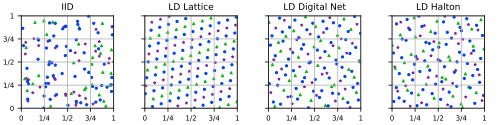
\includegraphics[width=1\linewidth,height=\textheight,keepaspectratio,alt={IID points with gaps and clusters alongside LD pointsets which more evenly fill the space. IID and LD pointsets. Each of the three randomized LD sequences contain purple stars (initial 32 points), green triangles (next 32), and blue circles (subsequent 64). The lattice was randomly shifted; the digital net was randomized with nested uniform scrambling (Owen scrambling); the Halton pointset was randomized with linear matrix scrambling and permutation scrambling.}]{../demos/talk_paper_demos/JOSS2025/JOSS2025.outputs/points.png}
\caption{IID points with gaps and clusters alongside LD pointsets which
more evenly fill the space. IID and LD pointsets. Each of the three
randomized LD sequences contain purple stars (initial 32 points), green
triangles (next 32), and blue circles (subsequent 64). The lattice was
randomly shifted; the digital net was randomized with nested uniform
scrambling (Owen scrambling); the Halton pointset was randomized with
linear matrix scrambling and permutation scrambling.\label{fig:points}}
\end{figure}

While (Q)MC methods are well established
\citep{dick2010digital, dick2013high}, practical implementation demands
numerical and algorithmic expertise. Our \texttt{QMCPy} implementation
follows MATLAB's Guaranteed Automatic Integration Library (GAIL)
\citep{ChoEtal21a2, TonEtAl22a}, with both softwares adhering to
reproducible research practices \citep{Cho14a2, ChoEtal22a}. However,
\texttt{QMCPy} consolidates a substantially broader range of
cutting-edge (Q)MC algorithms
\citep{ChoEtal22a, ChoEtal24a, sorokin2022bounding, sorokin2025unified, HicKirSor26a}
into a unified framework, bridging theory and practice, with the
following features:

\begin{itemize}
\tightlist
\item
  \textbf{Intuitive APIs} for problem specification and accessing (Q)MC
  methods,
\item
  \textbf{Flexible integrations} with \texttt{NumPy}
  \citep{harris2020array} and \texttt{SciPy} \citep{2020SciPy-NMeth},
\item
  \textbf{Robust and adaptive sampling} with theoretically grounded
  error estimation, and
\item
  \textbf{Extensible OO components} enabling researchers to implement
  and test new algorithms.
\end{itemize}

Unlike other (Q)MC modules such as \texttt{SciPy}'s
\texttt{scipy.stats.qmc} \citep{2020SciPy-NMeth} or \texttt{PyTorch}'s
\texttt{torch.quasirandom} \citep{NEURIPS2019_9015}, \texttt{QMCPy}
provides:

\begin{itemize}
\tightlist
\item
  customizable LD sequences with diverse randomization techniques,
\item
  rigorous adaptive error estimation algorithms, and
\item
  automatic variable transformations for (Q)MC compatibility.
\end{itemize}

\section{Components}\label{components}

(Q)MC methods approximate the multivariate integral
\begin{equation}\label{eq:mu-general}
\mu := \int_{\mathcal{T}} g(\mathbf{t}) \, \lambda(\mathbf{t}) \, d\mathbf{t},
\end{equation} where \(g\) is the \textbf{integrand} and \(\lambda\) a
non-negative weight. If \(\lambda\) is the probability density for a
random variable \(\mathbf{T}\), then
\(\mu = \mathbb{E}[g(\mathbf{T})]\), where \(\mathbf{T}\) is called the
\textbf{true measure}. Through an appropriate transformation
\(\boldsymbol{\psi}\), we rewrite \(\mu\) as the expectation of a
function of a standard uniform random variable \(\mathbf{X}\) over the
unit hypercube: \begin{equation}\label{eq:mu-uniform}
\mu = \mathbb{E}[f(\mathbf{X})] = \int_{[0,1]^d} f(\mathbf{x}) \, d\mathbf{x}, \qquad \mathbf{X} \sim \mathcal{U}[0,1]^d.
\end{equation}

If \(\boldsymbol{\psi}\) satisfies \(\mathbf{T} \sim
\boldsymbol{\psi}(\mathbf{X})\), then \(f = g \circ \boldsymbol{\psi}\).
This transformation accommodates IID and LD samples which are
approximately uniform on \([0,1]^d\).

(Q)MC methods estimate the population mean \(\mu\) in
\eqref{eq:mu-uniform} via the sample mean
\begin{equation}\label{eq:mu-hat}
\widehat{\mu} := \frac{1}{n} \sum_{i=1}^{n} f(\mathbf{X}_i).
\end{equation}

MC methods choose IID sampling nodes \(\mathbf{X}_1,\dots,\mathbf{X}_n\)
and have error \(|\widehat{\mu}-\mu|\) like \(\mathcal{O}(n^{-1/2})\)
\citep{Nie78}. QMC methods choose dependent LD nodes that fill
\([0,1]^d\) more evenly, achieving errors like
\(\mathcal{O}(n^{-1+\delta})\) where \(\delta>0\) is arbitrarily small
\citep{WanHic00b, Wan03a}. A key feature of \texttt{QMCPy} is
\textbf{stopping criteria} that automatically determine \(n\) so
\(|\mu - \widehat{\mu}| \le \varepsilon\) for a user-specified tolerance
\(\varepsilon>0\), either deterministically or with high probability.

\texttt{QMCPy} contains four main abstract classes which are extensible
for new (Q)MC algorithms:

\textbf{Discrete Distributions} generate IID or LD sampling nodes.
Available LD pointsets include lattices
\citep{Ric51, coveyou1967fourier, WanHic02a}, digital nets
\citep{Nie87, Nie92, DicPil10a} (including Sobol' \citep{Sob67}), and
Halton sequences \citep{Hal60}. We also support

\begin{itemize}
\item
  robust randomization routines \citep{sorokin2025unified}, including

  \begin{itemize}
  \tightlist
  \item
    \textbf{Lattices} with random shifts \citep{CraPat76, HicEtal03}.
  \item
    \textbf{Digital Nets} with digital shifts
    \citep{dick2005multivariate}, linear matrix scrambling (LMS)
    \citep{Mat98}, or nested uniform scrambling (NUS, also called Owen
    scrambling) \citep{Owe95, owen2003variance, dick2011higher}.
  \item
    \textbf{Halton Pointsets} with digital shifts \citep{WanHic00},
    permutation scrambling \citep{MorCaf94}, LMS
    \citep{Mat98, owen2024gain}, or NUS \citep{owen2024gain}.
  \end{itemize}
\item
  higher-order digital nets and higher order scrambling for integrands
  \(f\) with \(\alpha\) degrees of ``smoothness'', enabling QMC
  convergence like \(\mathcal{O}(n^{-\alpha+\delta})\) where
  \(\delta>0\) is arbitrarily small \citep{dick2011higher}.
\item
  custom generating vectors for lattices and generating matrices for
  digital nets, available from the growing collection in the
  \texttt{LDData} repository \citep{LDData}, which standardizes data
  from the Magic Point Shop \citep{KuoNuy16a} and Kuo's websites on
  lattices \citep{cools2006constructing, nuyens2006fast, KuoGenerators}
  and Sobol' points
  \citep{JoeKuo03, joe2008constructing, SobolDirection}.
\end{itemize}

Internally, our LD generators call our C package \texttt{QMCToolsCL}
\citep{QMCToolsCL}.

\textbf{True Measures} \(\mathbf{T}\) come with default transformations
\(\boldsymbol{\psi}\) satisfying
\(\boldsymbol{\psi}(\mathbf{X}) \sim \mathbf{T}\) where
\(\mathbf{X} \sim \mathcal{U}[0,1]^d\). For example, suppose
\(\mathbf{T}
\sim \mathcal{N}(\mathbf{m},\Sigma)\) is a \(d\)-dimensional Gaussian
random variable with mean \(\mathbf{m}\) and covariance \(\Sigma =
\mathbf{A}\mathbf{A}^T\). Then
\(\boldsymbol{\psi}(\mathbf{X}) = \mathbf{A}
\Phi^{-1}(\mathbf{X}) + \mathbf{m}\) where \(\Phi^{-1}\) is the inverse
distribution function of a standard normal applied elementwise. We
support many measures, including those from \texttt{SciPy}'s
\texttt{scipy.stats} \citep{2020SciPy-NMeth}.

\textbf{Integrands} \(g\), given a true measure \(\mathbf{T}\) and
transformation \(\boldsymbol{\psi}\), define the transformed integrand
\(f = g \circ
\boldsymbol{\psi}\) so that \(\mu = \mathbb{E}[g(\mathbf{T})] =
\mathbb{E}[f(\mathbf{X})]\) where
\(\mathbf{X} \sim \mathcal{U}[0,1]^d\). This change of variables is
performed automatically. Users only need to specify \(g\) and
\(\mathbf{T}\).

\textbf{Stopping Criteria (SC)} adaptively increase the sample size
until (Q)MC estimates satisfy user-defined error tolerances
\citep{HicEtal18a, TonEtAl22a, owen2024error}. SC vary depending on
properties of \(f\), and can include guaranteed MC algorithms
\citep{HicEtal14a} or QMC algorithms based on:

\begin{enumerate}
\def\labelenumi{\arabic{enumi}.}
\tightlist
\item
  multiple randomizations of LD pointsets \citep{l2023confidence},
\item
  quickly tracking the decay of Fourier coefficients
  \citep{HicRazYun15a, HicJim16a, JimHic16a, HicEtal17a, DinHic20a}, or
\item
  efficient Bayesian cubature by inducing structured Gram matrices
  \citep{Jag19a, RatHic19a, JagHic22a}.
\end{enumerate}

\texttt{QMCPy} is also capable of simultaneously approximating functions
of multiple integrands \citep{sorokin2022bounding}. Inspired by Julia's
\texttt{MultilevelEstimators.jl} \citep{MultilevelEstimators},
\texttt{QMCPy} is expanding support for multilevel (Q)MC SC
\citep{giles2009multilevel, giles2015multilevel} which exploit cheaper
low-fidelity surrogates to accelerate estimates of expensive integrands,
often in high or infinite dimensions.

\autoref{fig:stopping_crit} compares MC and QMC SC performance for
adaptively estimating the fair price of an Asian option across 100
trials per error tolerance. Both methods consistently meet tolerances.
The left panel shows sample complexity: MC algorithms require
\(n = \mathcal{O}(1/\varepsilon^2)\) samples while QMC algorithms
require only \(n = \mathcal{O}(1/\varepsilon)\) samples, with shaded
regions showing 10\%-90\% quantiles. The middle panel displays the
computation time, highlighting that QMC methods are much faster than MC
methods. The right panel presents error distributions via violin plots,
showing that the average error performance is better for QMC methods.

\begin{figure}
\centering
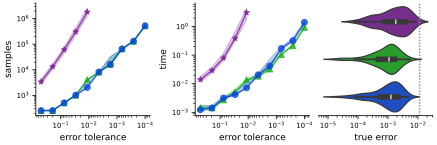
\includegraphics[width=1\linewidth,height=\textheight,keepaspectratio,alt={MC and QMC SC comparison for pricing of an Asian option. }]{../demos/talk_paper_demos/JOSS2025/JOSS2025.outputs/stopping_crit.png}
\caption{MC and QMC SC comparison for pricing of an Asian option.
\label{fig:stopping_crit}}
\end{figure}

\section{Distribution and Resources}\label{distribution-and-resources}

\texttt{QMCPy} can be installed using the command
\texttt{pip\ install\ qmcpy} \citep{qmcpy_pypi}. \autoref{fig:points}
and \autoref{fig:stopping_crit} are reproducible via the Jupyter
Notebook \citep{QMCPyJOSS2025Notebook}. Our project website
\citep{QMCBlog} features publications, presentations, blogs,
documentation \citep{QMCPyDocs}, and demos. Our GitHub repository
\citep{choi2023qmcpy} contains open-source code, tests, and issue
tracking \citep{ChoEtal22a, sorokin2025unified}. \texttt{QMCPy} is
distributed under the Apache (v2.0) license. Community feedback and
engagement are welcome.

\section{Acknowledgements}\label{acknowledgements}

The authors acknowledge support from the U.S. National Science
Foundation grant DMS-231601 and Department of Energy Office of Science
Graduate Student Research Program. We thank the international (Q)MC
research community for invaluable feedback and support.

\paragraph{Sign off here when you are satisfied with our
manuscript:}\label{sign-off-here-when-you-are-satisfied-with-our-manuscript}

\begin{itemize}
\tightlist
\item
  Aleksei G. Sorokin
\item
  Aadit Jain
\item
  Pieterjan Robbe
\item
  Sou-Cheng T. Choi
\end{itemize}

\bibliographystyle{abbrvnat}
\bibliography{refs_all}
\end{document}
